\chapter{Test}

\section{Unit test}
Her testes, om terningerne følger den givne stokastiske variabel.

Her testes, om der er lige stor sandsynlighed for at vinde, når man er spiller 1 og spiller 2.

\section{Coverage test}
Coverage test (\textit{dansk: kodedækningstekst}) omhandler metoderne i ens program.
Testen går såmænd ud på, at spillet bliver kørt, og den registrerer, hvorvidt alle metoderne bliver brugt, eller om der er såkaldt død kode, der ikke bliver brugt i nogle sammehænge.
Code coverage måles i en procentsats, og det betragtes ud fra normale omstændigheder som acceptabelt, at programmets code coverage er på 70-80\% \footnote{Cornett, Steve; Minimum Acceptable Code Coverage, http://www.bullseye.com/minimum.html, last updated: 2013. }.
Årsagen til den tilsynelagende lave acceptable code coverage skyldes, at det kan være for tidskrævende at få en højere procentsats.
I sikkerhedssystemer vil man dog normalt bestræbe sig efter 100\% code coverage.
\\
Vi har brugt IntelliJs integreret code coverage-test, som ligesom Eclipses code coverage-plugin viser, efter endt program, de forskellige procentsatser på de forskellige klasser. En enkel kørsel af spillet viser nedenstående resultat (kun spillet er testet, ikke GUI'en, som har en masse metoder, som ikke bliver benyttet):
\begin{figure}
    \begin{center}
        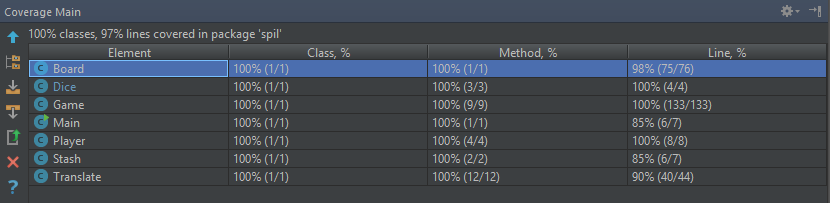
\includegraphics[width=15cm]{graphics/coveragetest/coveragetest1.png}
        \caption{Screen dump af code coverage}
        \label{fig:codecoverage}
    \end{center}
\end{figure}
\\ \\
Det fremgår af skærmbilledet, at alle procentsatser er >80\%, som der i større applikationer antages som acceptabelt. Ved at se, hvorfor nogle metoder ikke bliver brugt, så kan man ved at dykke ind i klasserne se, at eksempelvis bliver main-metoden i Main-klassen ikke bliver brugt. Ligeledes bliver der i Stash-klassen ikke brugt hele \textit{addAmount}-metoden, som det fremgår af skærmbilledet nedenunder:
\begin{figure}
    \begin{center}
        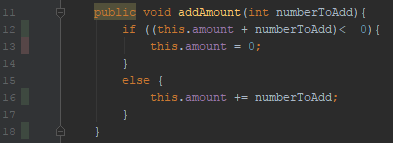
\includegraphics[width=8cm]{graphics/coveragetest/coveragetest2.png}
        \caption{Screen dump af addAmount}
        \label{fig:codecoverage_addamount}
    \end{center}
\end{figure}

\section{Testcases}

Vi har udarbejdet en række test cases ud fra kravende som er specificeret i kapitel \ref{sec:requirements}.
Disse test cases bekræfter at kravende er overholdt og programmet kan derfor godkendes bl.a. ud fra disse tests.

\begin{table}[H]
    \begin{center}
        \begin{tabular}{|l|p{8cm}|}
            \hline
            \textbf{Unique ID} & TC1 \\
            \hline
            \textbf{Summary} & Kan programmet modtage de korrekte navne? \\
            \hline
            \textbf{Requirements} & \\
            \hline
            \textbf{Preconditions} & \\
            \hline
            \textbf{Postconditions} & \\
            \hline
            \textbf{Procedure} & \begin{enumerate}
                \setlength\itemsep{0ex}
                \item Start spillet
                \item Indtast navnet "Abrahm" og tryk ok
                \item Indtast navnet "Kirsten" og tryk ok
            \end{enumerate} \\
            \hline
            \textbf{Test data} & \begin{itemize}
                \setlength\itemsep{0ex}
                \item Navn 1: Abraham
                \item Navn 2: Kirsten
            \end{itemize} \\
            \hline
            \textbf{Expected result} & Spillerne er blevet oprettet med navn og vises på brættet \\
            \hline
            \textbf{Actual result} & Som forventet \\
            \hline
            \textbf{Status} & Godkendt \\
            \hline
            \textbf{Tested by} & Magnus Hansen \\
            \hline
            \textbf{Date} & 10/11-2017 \\
            \hline
            \textbf{Environment} & IntelliJ on macOS \\
            \hline
        \end{tabular}
    \end{center}
    \caption{Test case 1 - test af navn}
    \label{tc:1}
\end{table}

\begin{table}[H]
    \begin{center}
        \begin{tabular}{|l|p{8cm}|}
            \hline
            \textbf{Unique ID} & TC2 \\
            \hline
            \textbf{Summary} & Kan spilleren kaste med terningerne? \\
            \hline
            \textbf{Requirements} & \\
            \hline
            \textbf{Preconditions} & TC1 \\
            \hline
            \textbf{Postconditions} & \\
            \hline
            \textbf{Procedure} & \begin{enumerate}
                \setlength\itemsep{0ex}
                \item Tryk på knappen "kast"
            \end{enumerate} \\
            \hline
            \textbf{Test data} & \\
            \hline
            \textbf{Expected result} & Det forventes at terningerne bliver kastet og vises på brættet \\
            \hline
            \textbf{Actual result} & Som forventet \\
            \hline
            \textbf{Status} & Godkendt \\
            \hline
            \textbf{Tested by} & Magnus Hansen \\
            \hline
            \textbf{Date} & 10/11-2017 \\
            \hline
            \textbf{Environment} & IntelliJ on macOS \\
            \hline
        \end{tabular}
    \end{center}
    \caption{Test case 2 - test af kast med terninger}
    \label{tc:2}
\end{table}

\begin{table}[H]
    \begin{center}
        \begin{tabular}{|l|p{8cm}|}
            \hline
            \textbf{Unique ID} & TC3 \\
            \hline
            \textbf{Summary} & Vil spillerens pengebeholdning opdateres i forhold til det felt han/hun rammer? \\
            \hline
            \textbf{Requirements} & \\
            \hline
            \textbf{Preconditions} & TC1 og TC2 \\
            \hline
            \textbf{Postconditions} & \\
            \hline
            \textbf{Procedure} & \begin{enumerate}
                \setlength\itemsep{0ex}
                \item Tjek at det rette felt rammes
                \item Tjek om pengebeholdning opdateres
            \end{enumerate} \\
            \hline
            \textbf{Test data} & \\
            \hline
            \textbf{Expected result} & Det forventes at spilleren rammer det rette felt og få tildelt/frataget penge fra pengebeholdningen i forhold til tabel \ref{table:fields} \\
            \hline
            \textbf{Actual result} & Som forventet \\
            \hline
            \textbf{Status} & Godkendt \\
            \hline
            \textbf{Tested by} & Magnus Hansen \\
            \hline
            \textbf{Date} & 10/11-2017 \\
            \hline
            \textbf{Environment} & IntelliJ on macOS \\
            \hline
        \end{tabular}
    \end{center}
    \caption{Test case 3 - Felt \& pengebeholdning}
    \label{tc:3}
\end{table}

\begin{table}[H]
    \begin{center}
        \begin{tabular}{|l|p{8cm}|}
            \hline
            \textbf{Unique ID} & TC4 \\
            \hline
            \textbf{Summary} & Vinder man ved en pengebeholdning på 3000 eller større? \\
            \hline
            \textbf{Requirements} & \\
            \hline
            \textbf{Preconditions} & TC1 \\
            \hline
            \textbf{Postconditions} & \\
            \hline
            \textbf{Procedure} & \begin{enumerate}
                \setlength\itemsep{0ex}
                \item Spil spillet for begge spillere.
            \end{enumerate} \\
            \hline
            \textbf{Test data} & \\
            \hline
            \textbf{Expected result} & Når en spiller rammer en pengebeholdning på 3000 eller mere, er vinderen funder og spillet afsluttes ved at vise et scoreboard \\
            \hline
            \textbf{Actual result} & Som forventet \\
            \hline
            \textbf{Status} & Godkendt \\
            \hline
            \textbf{Tested by} & Magnus Hansen \\
            \hline
            \textbf{Date} & 10/11-2017 \\
            \hline
            \textbf{Environment} & IntelliJ on macOS \\
            \hline
        \end{tabular}
    \end{center}
    \caption{Test case 4 - Vinder \& scoreboard}
    \label{tc:4}
\end{table}